\documentclass[12pt,letter]{exam}
\usepackage{graphicx}
\graphicspath{ {./img/ } }
\printanswers

\usepackage{hyperref}
\usepackage[
    type={CC},
    modifier={by-nc-sa},
    version={3.0},
    ]{doclicense}

\def\frontmatter{%
    \pagenumbering{roman}
    \setcounter{page}{1}
    \renewcommand{\thesection}{\Roman{section}}
}%

\def\mainmatter{%
    \pagenumbering{arabic}
    \setcounter{page}{1}
    \setcounter{section}{0}
    \renewcommand{\thesection}{\arabic{section}}
}%

\title{Pre-Nitrox Workbook}
\author{Maxwell Wenger}

\begin{document}
\maketitle

\frontmatter
\section{Licence}
\doclicenseThis

\section{Acknowledgements}
Special thanks to Tro Ota who helped edit and refine many of the questions in this document.

\section{Contact}
Humans are fallible. This document may not be free from errors. If you find any errors or have any suggestions, please let me know.
For comments, suggestions, or inquires, you will find my relevant contact information at https://github.com/maxwenger

\section{Preface}
This workbook is designed to help prepare you to take a recreational nitrox class. It covers the various subjects you will need a basic understanding to get the most out of that class. This is not designed to be an exam in any way, merely a tool to refresh your skills or remind you of topics you may have forgotten.

If you do not understand any concepts, please make a note of them as topics to brush up on before your nitrox class. Use this workbook as a reference, then use any and all resources, including your instructor, to find the correct answer. The point is not to see what you get wrong, but to understand all the subjects being covered.

This document is not meant to be a scuba training guide. Please seek out an active dive instructor that is affiliated with an RSTC approved dive agency for full and complete training.

\pagebreak

\mainmatter
\section{Math}
\begin{questions}
    \question Convert the following decimal numbers to percentages.
    \begin{parts}
        \part 0.2
        \part 0.21
        \part 0.84
        \part 0.843
        \part 1
        \part 1.2438
        \part 10.8
	\end{parts}
    \begin{solution}
        \begin{parts}
            \part 20\%
            \part 21\%
            \part 84\%
            \part 84.3\%
            \part 100\%
            \part 124.38\%
            \part 1080\%
	    \end{parts}
    \end{solution}
    \question Convert the following percentages to decimals.
    \begin{parts}
        \part 20\%
        \part 32\%
        \part 89.2\%
        \part 86.48\%
        \part 100\%
        \part 120.138\%
        \part 6100.9\%
	\end{parts}
    \begin{solution}
        \begin{parts}
            \part 0.2
            \part 0.32
            \part 0.892
            \part 0.8648
            \part 1
            \part 1.20138
            \part 61.009
	    \end{parts}
    \end{solution}
    \question Calculate the following.
    \begin{parts}
        \part $1\cdot 0.5$
        \part $1\cdot 1.5$ 
        \part 200\% of 1
        \part 132\% of 8
        \part 96\% of 6
        \part $16\cdot 0.46$
        \part $87\cdot 1.67$
        \part 100\% of 24
	\end{parts}
    \begin{solution}
        \begin{parts}
            \part 0.5
            \part 1.5
            \part 1
            \part 10.56
            \part 5.76
            \part 7.36
            \part 145.29
            \part 24
	    \end{parts}
    \end{solution}
    \question When you multiply a number by a factor that is less than one, the product will be \fillin the original number.

    \begin{oneparcheckboxes}
        \choice greater than
        \CorrectChoice less than
        \choice equal to
    \end{oneparcheckboxes}
    \question When you multiply a number by a factor that is greater than one, the product will be \fillin the original number.

    \begin{oneparcheckboxes}
        \CorrectChoice greater than
        \choice less than
        \choice equal to
    \end{oneparcheckboxes}
    \question 100\% of a number is \fillin the original number.

    \begin{oneparcheckboxes}
        \choice greater than
        \choice less than
        \CorrectChoice equal to
    \end{oneparcheckboxes}
    \question Solve for $x$.
    \begin{parts}
        \part $y = a + x$
        \part $y = a - x$
        \part $y = a \cdot x$
        \part $y = \frac{x}{a}$
        \part $y = \frac{a}{x}$
    \end{parts}
    \begin{solution}
        \begin{parts}
            \part $x = y - a$ 
            \part $x = a - y$
            \part $x = \frac{y}{a}$
            \part $x = y \cdot a$
            \part $x = \frac{a}{y}$
	    \end{parts}
    \end{solution}
\section{Units}
    \question Atmospheres, PSI, and bars, are all units of \fillin[pressure].
    \question 1 atmosphere of pressure is equal to \fillin[14.7] psi, and roughly equal to \fillin[1] bar.
    \question Roughly \fillin[33] ft, or \fillin[10] m of saltwater exerts 1 atmosphere of pressure.
    \question Roughly \fillin[34] ft, or \fillin[10.3] m of freshwater exerts 1 atmosphere of pressure.
    \question Calculate the pressure in atmospheres at each given depth of fresh water.
    \begin{parts}
        \part 34ft
        \part 84ft
        \part 184ft
        \part 34m
    \end{parts}
    \begin{solution}
        \begin{parts}
            \part 1ata
            \part 2.47ata
            \part 5.41ata
            \part 3.3bar 
        \end{parts}
    \end{solution}
    \question Calculate the pressure in atmospheres at each given depth of salt water.
    \begin{parts}
        \part 33ft
        \part 84ft
        \part 184ft
        \part 46m
    \end{parts}
    \begin{solution}
        \begin{parts}
            \part 1ata
            \part 2.55ata
            \part 5.58ata
            \part 4.6bar
        \end{parts}
    \end{solution}
\section{Physics}
    \question If I am properly weighted in freshwater, I will have to \fillin[add] weight for saltwater.
    \question The Atlantic ocean has a higher salinity than the Pacific ocean. If I am properly weighted for the Atlantic, I may have to \fillin[remove] weight to dive in the Pacific.
    \question You experience the greatest change in pressure going from the surface to 15ft of depth than going from 100ft to 115ft of depth.
    \begin{oneparcheckboxes}
        \CorrectChoice True
        \choice False
    \end{oneparcheckboxes}
    \question If you fill a balloon full of air on the surface, and take it to a depth of 33ft in seawater, the volume will \fillin[decrease] to a volume \fillin[50]\% of the original size, and the density of the gas will \fillin[increase] to a density that is \fillin[200]\% of the original density.
    \question If you fill a balloon full of air on the surface, and take it to a depth of 99ft in seawater, the volume will \fillin[decrease] to a volume \fillin[25]\% of the original size, and the density of the gas will \fillin[increase] to a density that is \fillin[400]\% of the original density.
    \question If you fill a balloon full of air at 33ft of depth in seawater, and take it to the surface, the volume will \fillin[increase] to a volume \fillin[200]\% of the original size, and the density of the gas will \fillin[decrease] to a density that is \fillin[50]\% of the original density.
    \question If you fill a balloon full of air at 132ft of depth in seawater, and take it to the surface, the volume will \fillin[increase] to a volume \fillin[500]\% of the original size, and the density of the gas will \fillin[decrease] to a density that is \fillin[20]\% of the original density.
    \question Air is \fillin[21]\% oxygen and \fillin[79]\% nitrogen.
\section{Physiology}
    \question Both oxygen and nitrogen are absorbed into your tissues, and can cause DCS if an unsafe amount of excess nitrogen and oxygen bubbles form inside your body due to decompression.

    \begin{oneparcheckboxes}
        \choice True
        \CorrectChoice False
    \end{oneparcheckboxes}
    \question Oxygen is an inert gas.

    \begin{oneparcheckboxes}
        \choice True
        \CorrectChoice False
    \end{oneparcheckboxes}
    \question \fillin gasses contribute to the bubbles that cause DCS.

    \begin{oneparcheckboxes}
        \choice All
        \CorrectChoice Only inert
        \choice All except inert
    \end{oneparcheckboxes}
 
    \question NDL stands for \fillin[No Decompression Limit].
    \question NDLs are a measure of \fillin[time].
    \question Dive tables calculate NDLs using two variables: \fillin[depth] and \fillin[bottom time].
    \question Based on the last question, fill in the following variables.
    \begin{parts}
        \part The \fillin[longer] or \fillin[deeper] the dive, the shorter the NDLs.
        \part The \fillin[shorter] or \fillin[shallower] the dive, the longer the NDLs.
    \end{parts}
    \question Describe the significance of NDLs to divers.
    \begin{solution}[1.5in]
       Answers may vary. Possible answer:
       NDLs are calculated using dive tables or a dive computer to determine the maximum allowable bottom time on a no decompression dive. Exceeding these limits greatly increases the risk of DCS.
    \end{solution}

        \question On-gassing is when our tissues \fillin[absorb] gasses.
        \question Off-gassing is when our tissues \fillin[release] gasses.

        \question At what point in the dive do you start to on-gas? \fillin[At the start of the descent.]
        \question At what point in the dive can you begin to off-gas? \fillin[At the start of the ascent.]
        \question At what point in the dive do your NDLs begin to count down? \fillin[At the start of the decent.]
        \question At what point in the dive do your NDLs stop counting down? \fillin[At the start of your ascent.]
        \question How do tables vary from computers in how they calculate NDLs?
        \begin{solution}[2in]
            Answers may vary. Dive tables do not take multilevel diving into account by default. Dive computers calculate multilevel profiles automatically.
        \end{solution}

\section{Dive Tables}
\textbf{For the following questions use the PADI RDP (if using the erdml or other tables your answers may be inaccurate)}

        \question Use the following graphic for all parts of this question.

        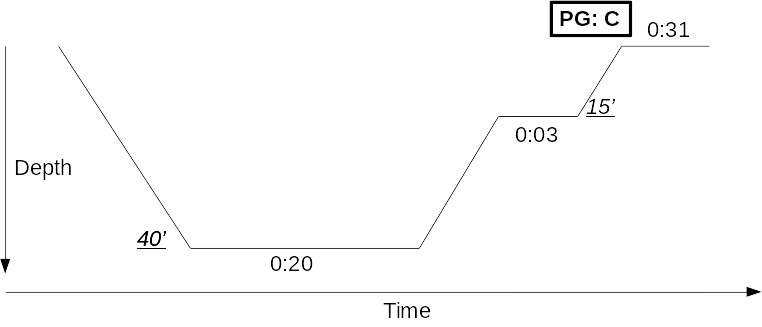
\includegraphics[width=\textwidth]{img/profile.png}
        \begin{parts}
            \part This diver's safety stop was \fillin[3] minutes long at \fillin[15] ft. 
            \part This diver's was in pressure group \fillin[C] after the dive.
            \part This diver did a \fillin[31] minute surface interval after the dive.
            \part This diver's bottom time was \fillin[20] minutes.
            \part This diver never exceeded a depth of \fillin[40] ft.
        \end{parts}

        \question Are safety stops always required? If not, when are they required?
        \begin{solution}[1.5in]
            A safety stop is not always required, but is always recommended. A safety stop is required when you come within three pressure groups of your NDL or on any dive deeper than 100ft.
        \end{solution}

        \question The NDL for a dive at 72ft is \fillin[30] minutes.
        \question You do a 34 minute dive to 63ft.
        \begin{parts}
            \part What is your pressure group? \fillin[Q]
            \part Is a safety stop required? \fillin[Yes]
            \part After this dive, how long of a SI is required before you are in PG K? \fillin[26] minutes.
        \end{parts}

        \question Your first dive is a 21 minute dive to 90ft. You do a 23 minute safety stop. Your second dive is a 28 minute dive to 54ft.
        \begin{parts}
            \part What is your pressure group after the first dive? \fillin[M]
            \part What is your pressure group after the surface interval? \fillin[I]
            \part What is your pressure group after the second dive? \fillin[V]
            \part Was a safety stop required for the first dive? \fillin[No]
            \part Was a safety stop required for the second dive? \fillin[Yes]
        \end{parts}

        \question Your initial pressure group is K.  What is your adjusted bottom time for a dive to 72 ft? \fillin[9] minutes.
        \question Your initial pressure group is Q. What is the minimum surface interval required to do a 58 minute dive to 41 ft? \fillin[64] minutes.

        \section{(Optional) Nitrox}
        \question Why do you want to learn how to dive nitrox?
        \begin{solution}[2in]
            Answers may vary.
        \end{solution}

\end{questions}
\end{document}
